%%----------------------------------------------------------
%% report_temp.tex
%% v1.0
%% 2022/10/28
%% by XIE Yuhao, e-mail: yuhaox@akane.waseda.jp
%%----------------------------------------------------------

\documentclass{wsdcr}

\title{IOT Based Smart Agriculture Monitoring System-Paper review}
\author{Aneesha.S}
\affil{Reg.No:21011101020\\
\textit{B.Tech Artificial intelligence and datascience}\\
\textit{Shiv nadar university-chennai}\\
E-mail: aneesha21110377@snuchennai.edu.in}
\date{22\textsuperscript{th} January, 2023}

\begin{document}

\maketitle

\section{Abstract}
\lettrine {F}{or }centuries, farming has been the main kind of employment in our nation. Agriculture is currently being hampered by the migration of people from rural to urban areas. Therefore, we use IoT-based smart agriculture solutions to solve this issue. This project comes with a number of features, including GPS-based remote control monitoring, moisture and temperature sensing, intruder frightening, security, leaf wetness, and appropriate irrigation capabilities. It uses wireless sensor networks to continuously record the characteristics of the soil and external variables. In different parts of the farm, different sensor nodes are installed. These characteristics can be controlled by any remote device or online services, and activities are carried out by connecting sensors, Wi-Fi, and cameras to microcontrollers. The wellbeing of the farmer is served by the creation of this idea as a product.


\section{Introduction to smart agriculture}
The goal of advancing agriculture is essential given the global trend toward new technology and their deployment. The field of agriculture is the subject of numerous studies. The majority of projects employ wireless sensor networks to gather data from numerous sensors placed at various nodes and transmit it using wireless protocol. The information about the numerous environmental elements is provided by the collected data. The best way to boost agricultural output is not solely to monitor environmental elements.
Numerous other factors also contribute to a greater degree of productivity loss. Therefore, automation needs to be used in agriculture to solve these issues.

Therefore, in order to address all of these issues, it is vital to create an integrated system that would address all aspects influencing productivity at every stage.
However, a number of problems prevent agriculture from becoming fully automated. Despite being used at the scientific level, it is not made available to farmers as a product so they can take advantage of the resources. Consequently, the topic of this study is providing farmers with IoT-based smart agriculture.



\begin{figure}[t!]
    \centering
    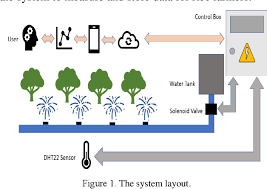
\includegraphics[width=.9\linewidth]{download.png}
    \caption{  A prototype of smart agriculture}
    \label{fig:example}
\end{figure}


\section{Literature Survey}
The manual approach of checking the parameters is still in use today and is one of the earliest methods in agriculture. The farmers themselves calculate the readings and verify all the parameters in this way. It focuses on creating gadgets and solutions that take advantage of wireless sensor network system benefits to manage, show, and alert users. It uses automation and IoT technology to make agriculture smart. Smart GPS-based remote controlled robots with the ability to identify humans and execute duties like spraying, weeding, and moisture monitoring are the standout characteristics.

The cloud computing tools can build a full computing system from sensors to tools that detect data from photographs of agricultural fields and from people on the ground and precisely feed the data into the repository together with the position as GPS coordinates. With the help of wireless communication technology, this concept links a smart sensing system and a smart irrigation system to create a revolutionary approach for smart farming. It suggests a low-cost and effective wireless sensor network method to collect soil moisture and temperature from different farm locations and according to the requirements of crop controllers to determine whether irrigation is enabled or not.  It puts forth a theory regarding how automated irrigation systems were created to maximise the use of water for agricultural crops.A gateway device additionally manages sensor data. Using Ethernet IEEE 802.3, the air conditions are monitored and managed online. You can use as much of the partial root zone drying process as possible. It is intended for Internet of Things (IoT)-based monitoring systems to study crop environments and the way to increase the effectiveness of decision-making by examining harvest information. In this study, image processing is employed as a method to track fruit disease outbreaks from planting through harvest. The variances can be apparent in morphology, colour, and texture. In this essay, a greenhouse is a structure where plants are grown in a protected atmosphere. It is employed for greenhouse management, data collection, and maintaining the ideal environmental conditions.

\section{Proposed work}
Different sensors, including temperature, moisture, and PIR sensors, are deployed in the field portion.
These sensors' data collection devices are linked to the microcontroller through RS232.
The received data is checked against the threshold values in the control section. The buzzer is turned on and the LED begins to flicker if the data is greater than the threshold value. After sensing, the power is automatically turned off and this alarm is conveyed to the farmer as a message. The values are generated on the website, and the farmer receives a thorough explanation of them.

In manual mode, the user must hit the button in the Android application created to turn the microcontroller ON and OFF. The GSM Module is used to accomplish this.
In automated mode, if the value reaches the threshold point, the microcontroller is automatically switched ON and OFF. A user alert must be automatically sent shortly after the microcontroller is turned on. This is done by using the GSM module to send the user a message.
The water level sensor is only used to show the amount of water in a tank or other water resource. Other metrics like temperature, humidity, moisture, and PIR sensors show the threshold value.



\section{About the Hardware used}
\subsection{PIC16F877A-microcontroller: }

One of the most widely used microcontrollers on the market is the PIC 16F877A. It is more manageable and user-friendly. This controller's coding and programming are both simple. The technology of flash memory makes it simple to erase the coded programme. The microcontroller is employed in a wide variety of significant sectors. It is utilised in industrial automations, remote sensing, residential appliances, and security. Another characteristic is an EEPROM, which is used to permanently store information such as broadcast and receive frequencies and other pertinent data.
\begin{figure}[t!]
    \centering
    \includegraphics[width=.9\linewidth]{image.png}
    \caption{ }
\subsection{ Architecture of PIC16F877A }
    \label{fig:example}
\end{figure}

\subsection{GSM module}
A GSM modem can function like a mobile phone with its own specific phone number and can accept any GSM network operator SIM. This must be used since it supports the RS-232 standard and can be quickly attached to the controller. It may be used as a phone by sending and receiving SMS and placing calls.

Through RS232, the GSM modem is linked to the controller. Using AT Commands, the SMS is transmitted from the terminal to the recipient number. The controller uses "AT-Attention" commands to direct the GSM to carry out the desired action. Additionally, it incorporates LED notifications and reverse voltage protection. It runs on the 900/1800 MHz band.
\begin{figure}[t!]
    \centering
    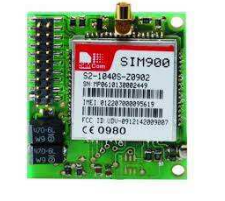
\includegraphics[width=.9\linewidth]{gsm.png}
    \caption{ }
\subsection{ GSM module }
    \label{fig:example}
\end{figure}

\subsection{Soil moisture sensor:}
Soil moisture sensor is a sensor which senses the moisture 
content of the soil. The sensor has both the analog and the 
digital output. The digital output is fixed and the analog 
output threshold can be varied. It works on the principle of 
open and short circuit. The output is high or low indicated 
by the LED. When the soil is dry, the current will not pass 
through it and so it will act as open circuit. Hence the output 
is said to be maximum. When the soil is wet, the current will 
pass from one terminal to the other and the circuit is said to 
be short and the output will be zero.
\begin{figure}[t!]
    \centering
    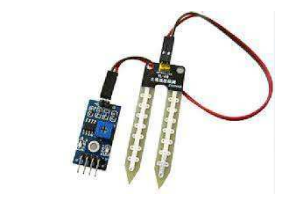
\includegraphics[width=.9\linewidth]{soil.png}
    \caption{ }
\subsection{ Soil moisture sensor }
    \label{fig:example}
\end{figure}
\subsection{Temperature sensor}
The LM 35 sensor is highly used because its output voltage 
is linear with the Celsius scaling of temperature. It does not 
provide any external trimming. It has a wide operating 
range. The maximum output is 5V. The output will increase 
10mV for every one degree rise in temperature. The range is 
from -55 degrees to +150 degrees. There are three terminals 
as Vcc, Ground and the analog sensor. It consumes 
minimum amount of electricity. Thus, it is energy efficient. 
It is very efficient in horticulture. It is user friendly to use. 
\begin{figure}[t!]
    \centering
    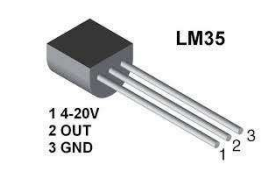
\includegraphics[width=.9\linewidth]{temp.png}
    \caption{ }
\subsection{ Temperature sensor }
    \label{fig:example}
\end{figure}
\subsection{PIR sensor}
Any object with a temperature greater than absolute zero radiates heat energy. It emits infrared wavelengths, making it invisible to the human eye. PIR sensors detect the infrared radiation that is released or reflected from an object rather than heat. It is employed to find moving individuals, animals, or other items.

They are frequently utilised in lighting control systems and burglar alarms. The temperature will increase from ambient temperature as a person walks by in the field. The sensor transforms the ensuing variation into a variation in the output voltage, which initiates the detection.
\begin{figure}[t!]
    \centering
    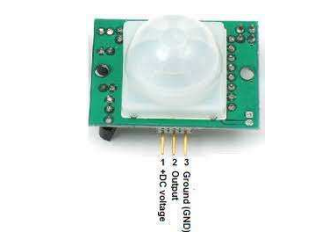
\includegraphics[width=.9\linewidth]{pir.png}
    \caption{ }
\subsection{ PIR sensor }
    \label{fig:example}
\end{figure}

\section{About the Software used}
\subsection{Proteus 8 simulator}
One of the greatest simulation programmes for different microcontroller circuit designs is Proteus 8. It is a widely used simulator since nearly all microcontrollers and electronic components are readily available in it.

Before actual hardware testing, it can be used to evaluate software and embedded designs for electronics. Proteus allows for the simulation of microcontroller programming. Through simulation, the danger of faulty design damaging hardware is reduced.

\section{Experimentation and result}
The hardware is interfaced with all the sensors in the board. 
The hardware components include the microcontroller, 
buzzer, relay, ADC converter, GSM module and all the 
sensors interfaced. The board is inserted with a SIM card 
which is used to communicate with the owner and the 
recorded values. 

The output shown below denotes the temperature, soil 
moisture condition and the intruder detection. The second 
result is the output from the Android Application that is 
developed in the mobile phone. It determines the 
temperature, humidity, moisture and the intruder detection.

\section{My view about the system}
Increased productivity, real-time monitoring, disease and pest detection, weather forecasting, water management, and remote access are just a few of the advantages that IOT-based smart agriculture monitoring systems provide farmers. These systems gather information on soil moisture, temperature, and other factors using a range of sensors and other technologies. This information may then be utilised to better plan when to sow and harvest crops. This may lead to higher agricultural yields and lower expenses, which would boost farmers' profitability.

These systems can also automate procedures like fertilising and watering plants, which lowers labour expenses and boosts productivity. Farmers may manage their farms from anywhere with the capacity to access and monitor the data gathered by smart systems remotely. Smart systems can also assist farmers in resource conservation by only watering crops when necessary and detecting early disease or pest indications, enabling them to take preventative actions before they cause serious harm.

Technology is a major component of smart agriculture systems, so if something goes wrong, farmers can be left without vital information on their crops. IoT-based agriculture systems' data gathering and utilisation presents privacy issues because the data may be gathered and shared with third parties without the farmer's knowledge. It can be challenging to integrate many systems and get them to function well together given the wide variety of sensors and software that are offered by numerous manufacturers. When internet connectivity is poor in rural regions, it can be challenging to get sensor data to farmers or other stakeholders.

The restricted catalogue of components in Proteus 8 can make it challenging to simulate more intricate circuits and systems. Compared to other simulation software, roteus 8 has fewer simulation capabilities. It might not be able to replicate specific circuit or system types. Due to Proteus 8's restricted debugging tools, it is challenging to find and correct simulation mistakes. The restricted possibilities for importing and exporting designs in roteus 8 can make it challenging to collaborate on or exchange designs made in other programmes.The ideal substitute is Circuit JS, which is both open source and free. QUCS, Autodesk EAGLE, OpenModelica, and Autodesk Tinkercad are some more excellent alternatives to proteus VSM.
Circuit simulators are the main proteus VSM alternatives, however CAD software or electronic design automation tools may also be used. If you want a more focused set of options or are looking for a certain proteus VSM functionality, you can filter by these.

Despite these difficulties, IoT-based smart agriculture monitoring systems have a lot of potential. These solutions are likely to gain more and more traction among farmers as technology advances and costs come down. Additionally, the usage of IoT-based smart agriculture monitoring systems may become more crucial in the coming years due to the growing need to address concerns like climate change and food security.


\section{Conclusion}
In conclusion, IoT-based smart agriculture monitoring systems offer a wide range of benefits for farmers, including increased efficiency, real-time monitoring, disease and pest detection, weather forecasting, water management, and remote access. However, these systems also have their drawbacks, including high costs, limited connectivity, and lack of standardization. Despite these challenges, the potential for IoT-based smart agriculture monitoring systems is significant, and as technology continues to improve, these systems are likely to become increasingly popular among farmers.

\section{References}
1.International Journal on Recent and Innovation Trends in Computing and Communication ISSN: 2321-8169,Volume: 5 Issue: 2.

2.www.alternativeito.net

3.www.libelia.com

4.google images 

5.ieee.org
\end{document}
